% !TeX root = ../../main.tex
\section{Model implementation}

COMSOL was selected for detailed reactor modelling

\subsection{Model equations}
COMSOL eqns

\subsection{Optimisation and sensitivity analysis}

\subsubsection{Secondary cooling system sizing}

\begin{figure}[h]
    \centering

    \begin{subfigure}{0.49\linewidth}
        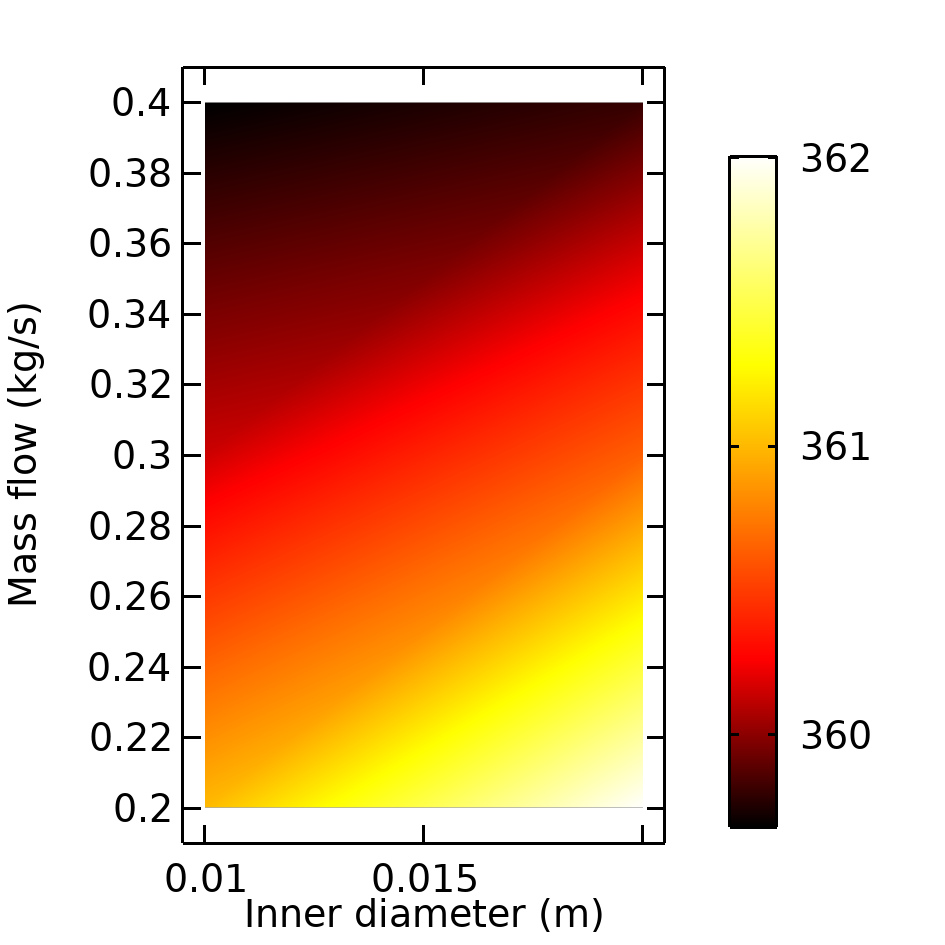
\includegraphics[width=\linewidth]{figures/S2-maxT.png}
        \caption{Maximum temperature reached in the reactor}
        \label{fig:comsol-S2:maxT}
    \end{subfigure}
    \begin{subfigure}{0.49\linewidth}
        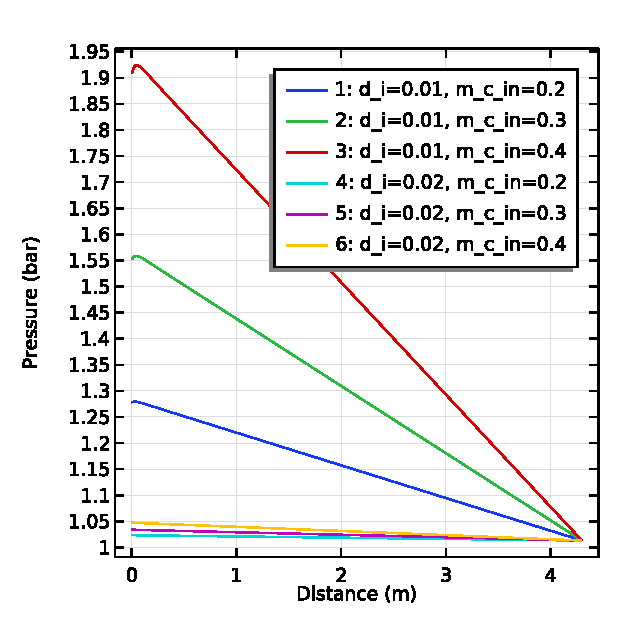
\includegraphics[width=\linewidth]{figures/S2-CW-Pdrop.eps}
        \caption{CW side pressure drop}
        \label{fig:comsol-S2:CW-Pdrop}
    \end{subfigure}

    \caption{Sensitivity to secondary CW parameters}
    \label{fig:comsol-S2}
\end{figure}
Inner coolant flowrate and diameter of inner cooling tube were optimised to keep temperature below the safe limit of 363K while maintaining a low pressure drop. As seen in Figure \ref{fig:comsol-S2:maxT}, it is desirable to have a small inner cooling tube diameter and a high coolant flowrate to keep the reactor temperature low. However, the smaller the diameter, the greater the increase in pressure drop per unit length as the coolant flowrate increases. This could be a problem in the future when the throughput is expected to increase when Nitroma's production grows. Thus, it is important to have a larger inner diameter that gives the flexibility of increasing inner coolant flowrate to remove heat from the reaction. Moreover, having a lower pressure drop means no high pressure pump is required to feed the cooling water into the reactor. The final determined values were inner diameter of 0.02m and inner coolant flowrate of 0.3 kg/s. At these specifications, the temperature of reactor can still be kept below 363K while keeping pressure drop to a minimum.

\subsubsection{Cocurrent vs counter-current cooling water flow}
[insert cocurrent vs countercurrent]
Cocurrent flow: CW warms the downstream end of the reactor, improving rate.

Countercurrent: CW removes heat from downstream section (slowing rate unneccesarily) and is then warm when it reaches the hotspot, limiting its usefulness in minimising the risk of thermal runaway.

\subsubsection{\ch{HNO3}:Toluene inlet ratio}

\begin{figure}[h]
    \centering
    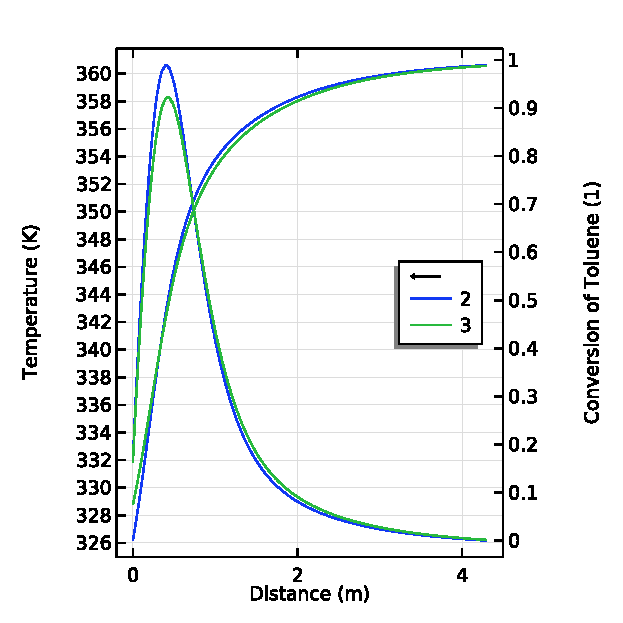
\includegraphics[width=0.49\linewidth]{figures/S3-T-X.eps}
    \caption{Effect of changing nitric acid molar ratio on temperature and conversion profiles in reactor.}
    \label{fig:comsol-S3-T-X}
\end{figure}

\ch{HNO3}:Toluene molar ratio of 2 and 3 were investigated to achieve 98\% conversion in the shortest reactor length possible. Nitric acid is always kept in excess to maximise the formation of nitronium ion on the catalyst surface. Conversely, if the toluene is in excess, it will block the acid sites on the catalyst which obstructs the formation of nitronium ions [vassena et al]. 

The results showed that increasing the \ch{HNO3}:Toluene molar ratio from 2 to 3 had negligible effect on the conversion of toluene. This suggests that the surface of the catalyst had already been fully saturated. Therefore, increasing molar flowrate of nitric acid further would not enhance the conversion of the nitration reaction, but would instead lead to higher OPEX costs of supplying nitric acid to the reactor. It could also complicate the separation process of the 3 nitrotoluene isomers downstream. 

As safety is one of the key priorities of Nitroma in all decision making, the maximum temperature in the reactor were also analysed for both cases before making a final decision. Both cases were found to be below the safe temperature limit of 363K, hence, a molar flowrate ratio of 2 was selected.

\subsubsection{Number of tubes}

\subsubsection{Pareto frontier}
MATLAB \texttt{gamultiobj}

\subsubsection{Coolant temperature}
Extra length to allow for variations in T

\subsection{Final results}
\begin{figure}[h]
    \centering
    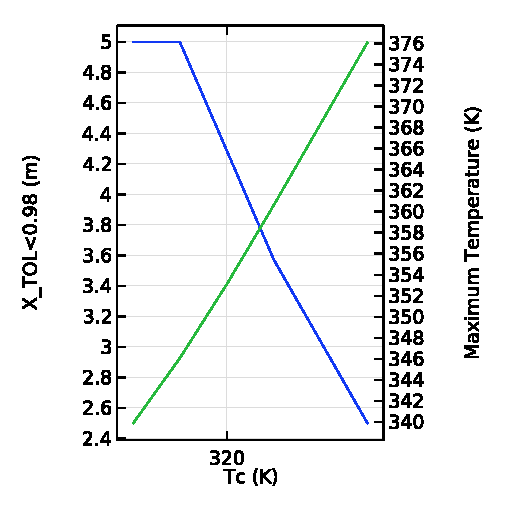
\includegraphics[width=0.49\linewidth]{figures/S4-CW-X-T.eps}
    \caption{Effect of CW temperature on distance required to reach 98\% conversion (blue) and max T (green)}
    \label{fig:comsol-S4-CW-X-T}
\end{figure}

\subsection{Final results}
The nitration reactor was robust after optimisation. 
The reactor sees a sharp rise in conversion (\approx 80\%) in the first 1m of reactor before achieving the remaining 20\% in the next approx 3m. This can be explained by the temperature variation as shown in Figure \ref{fig:comsol-temperature}. The reaction proceeds the most rapidly at the start of re
As expected, the more valuable ONT and PNT were produced in much greater amounts as compared to MNT. 

\begin{figure}[h]
    \centering

    \begin{subfigure}{0.49\linewidth}
        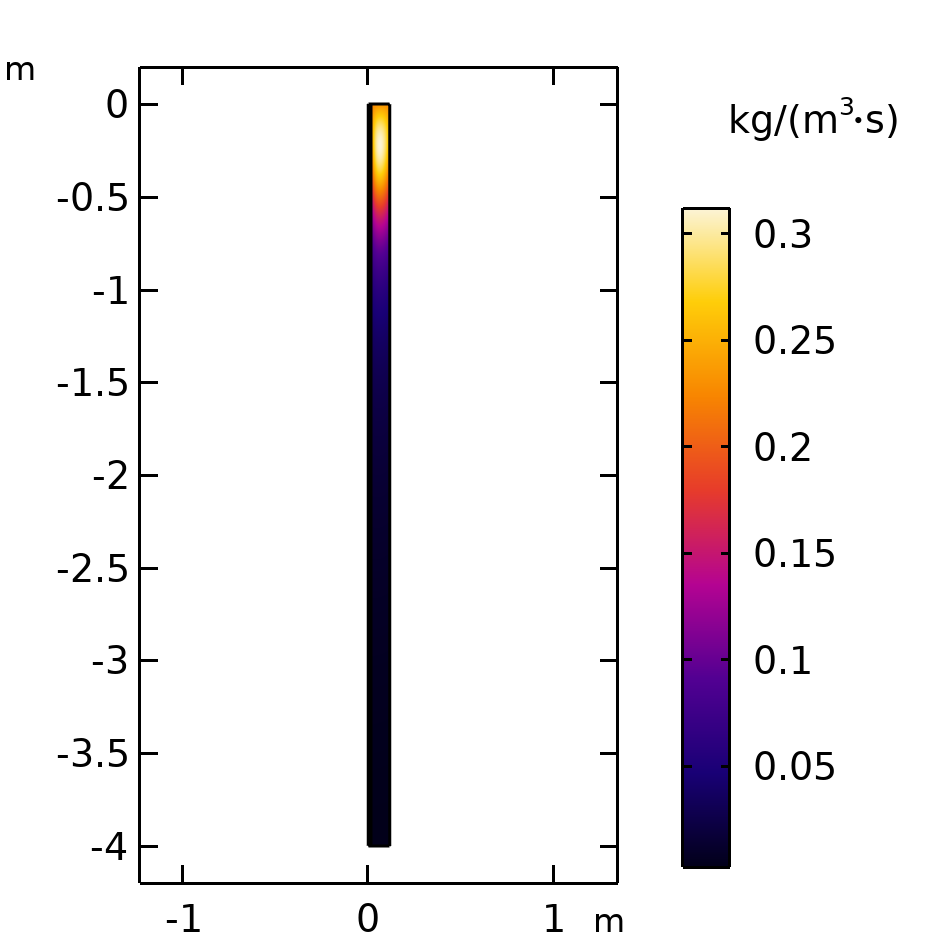
\includegraphics[width=\linewidth, scale=0.5]{figures/r_TOL.png}
        \caption{Rate of Toluene reaction}
        \label{fig:comsol-performance:r_TOL}
    \end{subfigure}
    \begin{subfigure}{0.49\linewidth}
        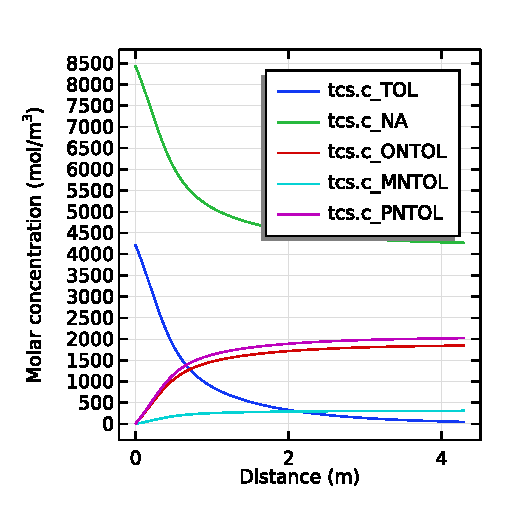
\includegraphics[width=\linewidth, scale=0.5]{figures/concentration.eps}
        \caption{Concentration profile within reactor}
        \label{fig:comsol-performance:concentration}
    \end{subfigure}

    \caption{Reactor performance}
    \label{fig:comsol-performance}
\end{figure}


See \cref{fig:comsol-conversion}.

\begin{figure}[h]
    \centering

    \begin{subfigure}{0.49\linewidth}
        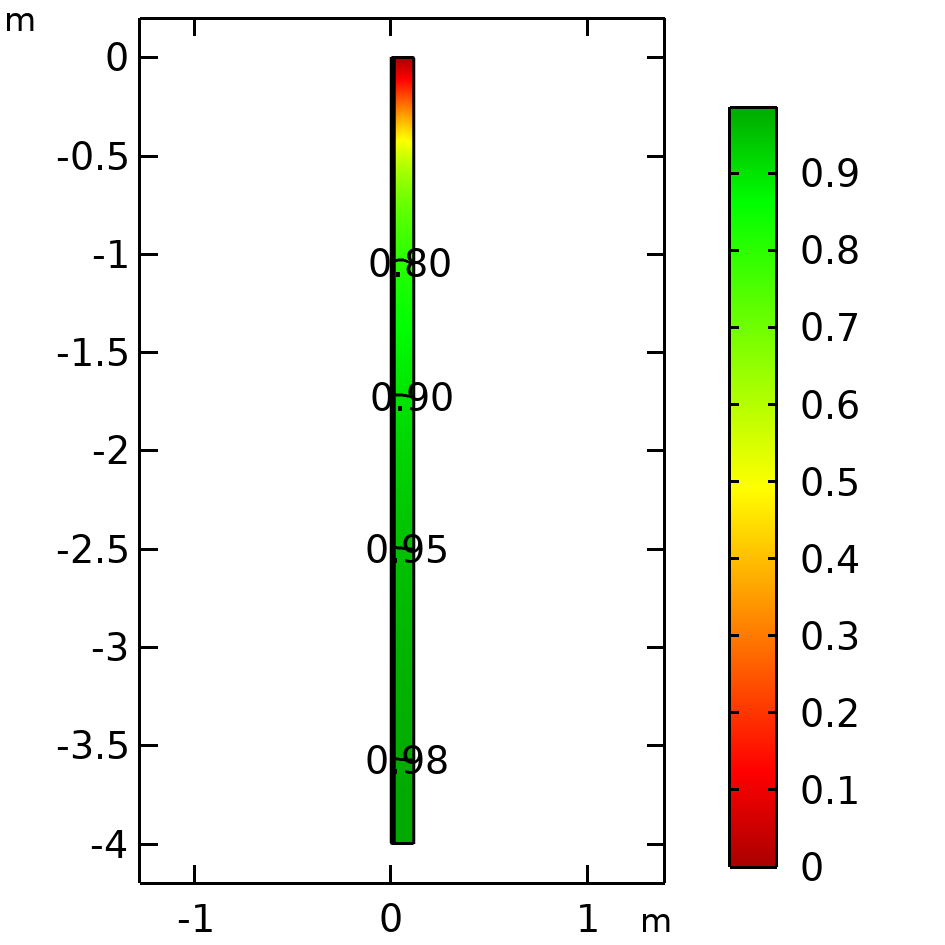
\includegraphics[width=\linewidth, scale=0.5]{figures/conversion-surface.png}

        \label{fig:comsol-conversion:surface}
    \end{subfigure}
    \begin{subfigure}{0.49\linewidth}
        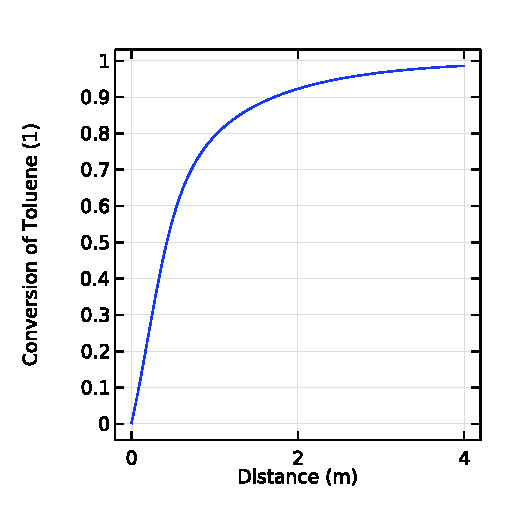
\includegraphics[width=\linewidth, scale=0.5]{figures/conversion-line.eps}

        \label{fig:comsol-conversion:line}
    \end{subfigure}

    \caption{Conversion of toluene across reactor length}
    \label{fig:comsol-conversion}
\end{figure}
The reaction achieves 98\% conversion in 3.6m 
\subsubsection{Temperature}
[include radial temp at max temp location]
See \cref{fig:comsol-temperature}.

\begin{figure}[h]
    \centering

    \begin{subfigure}{0.49\linewidth}
        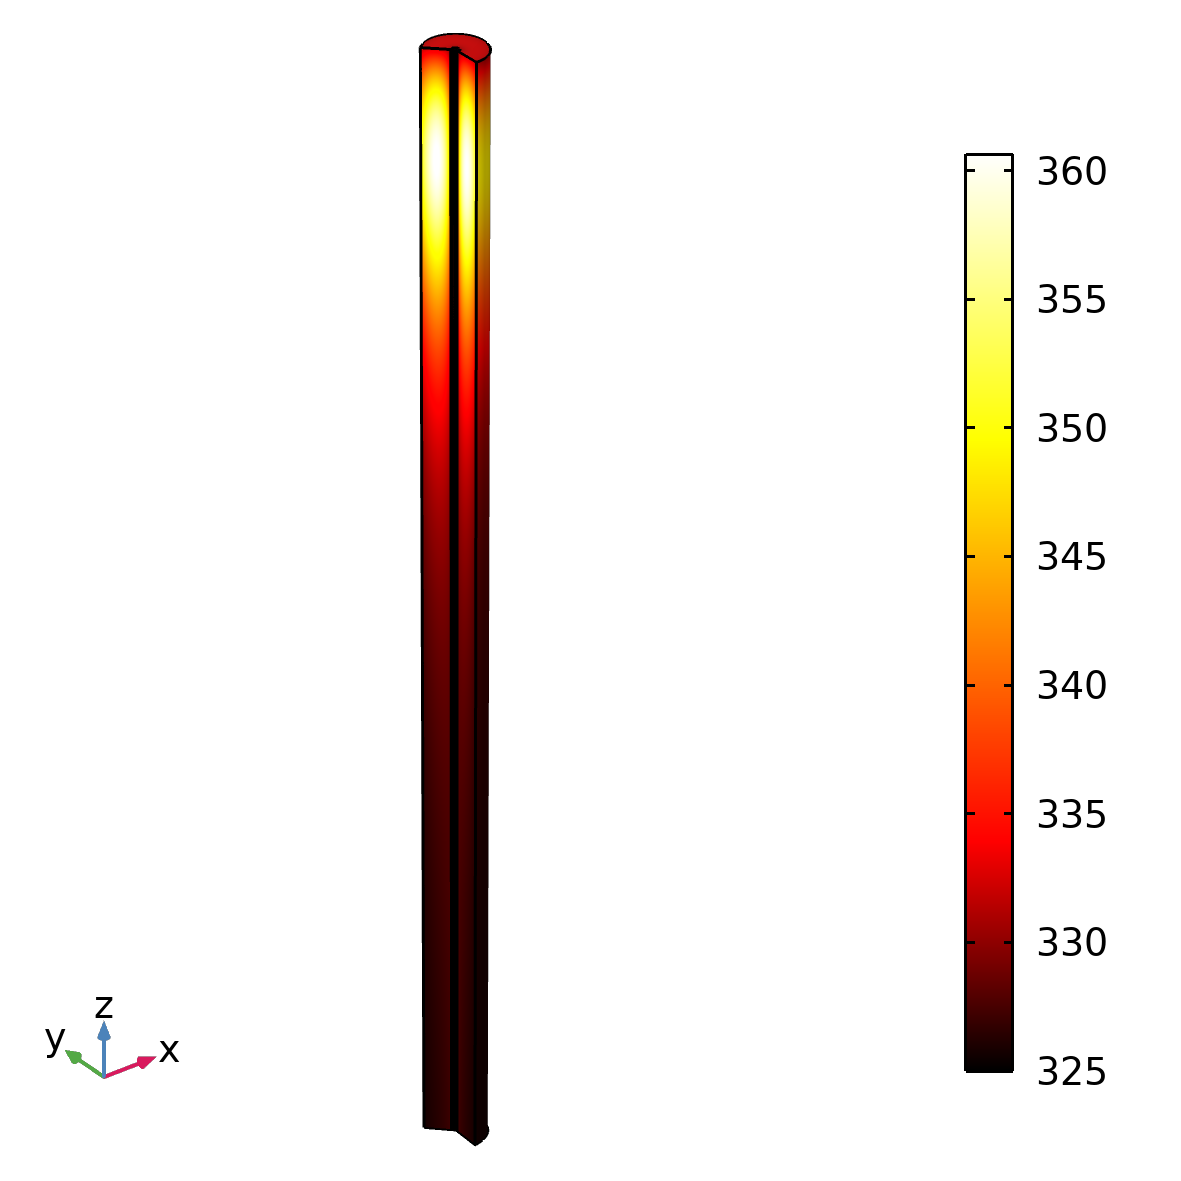
\includegraphics[width=\linewidth, scale=0.5]{figures/temperature-surface.png}
        \caption{}
        \label{fig:comsol-temperature:surface}
    \end{subfigure}
    \begin{subfigure}{0.49\linewidth}
        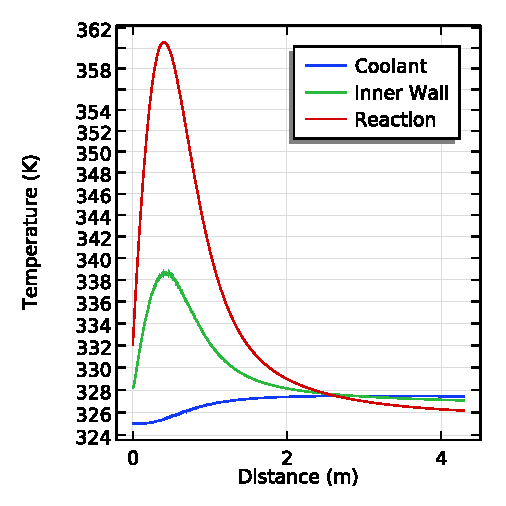
\includegraphics[width=\linewidth, scale=0.5]{figures/temperature-lines.eps}
        \caption{}
        \label{fig:comsol-temperature:lines}
    \end{subfigure}

    \caption{Temperatures}
    \label{fig:comsol-temperature}
\end{figure}
